\documentclass[conference]{IEEEtran}
\usepackage{cite}
\usepackage{amsmath,amssymb,amsfonts}
\usepackage{algorithmic}
\usepackage{graphicx}
\usepackage{textcomp}
\usepackage{xcolor}
\usepackage{booktabs}
\usepackage{float}
\usepackage{subcaption}
\usepackage{multirow}
\usepackage{url}

\begin{document}

\title{Deep Reinforcement Learning for AUV Depth Control: PPO/SAC vs PID Baseline with Domain Randomization Robustness Analysis}

\author{
\IEEEauthorblockN{Taimin Gong}
\IEEEauthorblockA{\textit{School of Computer Science and Information Security} \\
\textit{Guilin University of Electronic Technology}\\
Guilin 541004, China \\
taimin.gong@example.com}
\and
\IEEEauthorblockN{Xiaonan Luo}
\IEEEauthorblockA{\textit{School of Computer Science and Information Security} \\
\textit{Guilin University of Electronic Technology}\\
Guilin 541004, China \\
luoxn@guet.edu.cn}
}

\maketitle

\begin{abstract}
This paper addresses the depth control problem of autonomous underwater vehicles (AUVs) under complex disturbances, where traditional PID controllers often suffer from limited robustness. We evaluate two deep reinforcement learning (DRL) algorithms, PPO and SAC, against a grid-search-tuned PID baseline. A vertical-plane second-order dynamic Gymnasium environment is constructed, and a multi-objective reward function is designed to balance tracking accuracy, energy consumption, and action smoothness. Domain randomization over mass and drag coefficient is evaluated as a robustness training strategy. Comparative experiments are conducted among PID, PPO, and SAC under nominal, impulse-perturbed, and parameter-offset conditions. Results show that the DRL-based controllers match the tuned PID baseline in nominal tracking accuracy and significantly outperform it in disturbance rejection: pulse-trained policies maintain a hold ratio above 0.95 under impulse disturbances, while PID degrades notably. Training regime is the dominant factor in robustness: pulse-trained policies consistently improve hold ratio by approximately 0.7 percentage points across all evaluation conditions (paired Wilcoxon, $p < 0.001$), whereas PPO and SAC differ by less than 0.25 percentage points, and only under parameter offsets---suggesting that part of the algorithm-level conclusions in the literature may reflect uncontrolled evaluation variance rather than the algorithms themselves. Domain randomization, however, yields no benefit under the tested parameter offsets; it incurs a small but statistically significant degradation of approximately 0.6 percentage points (paired Wilcoxon, $p < 0.001$). Notably, the evaluation offsets ($+15\%$ mass, $-25\%$ drag) lie outside the randomization ranges used during training, suggesting that the robustness conferred by DR does not extrapolate beyond the trained parameter distribution in our setup. All paired per-episode evaluation data are publicly released to support reproducible comparison.
\end{abstract}

\begin{IEEEkeywords}
AUV, Deep Reinforcement Learning, Depth Control, Domain Randomization, PPO, SAC
\end{IEEEkeywords}

\section{Introduction}
Depth keeping is a foundational capability for autonomous underwater vehicles (AUVs) in seabed mapping, pipeline inspection, and long-endurance observation missions. The vertical-plane dynamics of an AUV are strongly coupled, nonlinear, and subject to hydrodynamic parameter uncertainty (e.g., estimated mass and drag) as well as external disturbances from currents and tether loads. Although classical PID controllers remain the engineering standard, their performance depends heavily on manual gain tuning and degrades under disturbances---in our experiments, the hold ratio of a grid-search-tuned PID drops by roughly 4 percentage points under injected force pulses.

Deep reinforcement learning (DRL) has recently been applied to AUV control~\cite{wu2017depth}, offering a model-free alternative that learns policies directly from interaction. However, two systematic shortcomings limit the interpretability of existing DRL-vs-classical comparisons. First, evaluation protocols are typically unpaired---methods are tested with different random seeds or initial conditions, so small but systematic effects are masked by initial-condition variance. Second, confounding variables are not isolated: conclusions such as ``algorithm A outperforms algorithm B'' frequently conflate the algorithm with the training regime (e.g., disturbance-injected training versus nominal training), making attribution impossible. In parallel, domain randomization (DR) has become a standard tool for sim-to-real transfer~\cite{tobin2017dr,peng2018}, yet its behavior under parameter offsets \emph{outside} the trained randomization range is rarely reported honestly.

In this work, we perform a variance-reduced, controlled comparison on a unified AUV vertical-plane depth-keeping environment. We adopt common-random-number pairing (seed 5678) with the paired Wilcoxon signed-rank test as the primary statistical test, and we isolate the training regime from algorithm choice by training both PPO and SAC under identical conditions. Our evaluation covers four scenarios: nominal, force-pulse, mass offset ($+15\%$), and drag offset ($-25\%$).

Our contributions are threefold:
\begin{itemize}
\item \textbf{A variance-reduced evaluation protocol.} We adopt common-random-number pairing with the paired Wilcoxon signed-rank test for DRL-vs-baseline comparison. The protocol resolves hold-rate differences below one percentage point---differences that are statistically indistinguishable from initial-condition noise under the unpaired protocols used in most prior comparisons---and we release all paired per-episode data to make the analysis reproducible.\footnote{Code, trained models, and all paired per-episode evaluation data are available at \url{https://github.com/gtm1354509080/auv-embodied-sim}.}
\item \textbf{An attribution finding: training regime, not algorithm choice, dominates robustness.} Disturbance-injected (force-pulse) training consistently improves hold ratio by approximately 0.7 percentage points across all four scenarios (paired Wilcoxon, $p<0.001$), whereas PPO and SAC differ by less than 0.25 percentage points, and only under parameter offsets. Because differences of this magnitude are below the resolution of unpaired evaluation, part of the algorithm-level conclusions in the literature may be attributable to uncontrolled evaluation variance rather than to the algorithms themselves.
\item \textbf{A reproducible negative result marking the boundary of domain randomization.} DR over mass $\pm10\%$ and drag $\pm20\%$ yields no benefit under offsets outside the trained ranges ($+15\%$ / $-25\%$), incurring a small but significant degradation ($\approx 0.6$ percentage points): in our setup, DR robustness does not extrapolate beyond the trained parameter distribution. The practical guidance is that DR randomization ranges must be chosen to cover the expected deployment deviations.
\end{itemize}

\section{Related Work}

\subsection{Classical AUV Depth Control}
Control of underwater vehicles has been studied for four decades. Yoerger and Slotine~\cite{yoerger1985robust} pioneered sliding-mode trajectory control for underwater vehicles, showing that robustness to imprecise models can be obtained with modest computation. Healey and Lienard~\cite{healey1993sliding} extended this line to a multivariable sliding-mode autopilot for the combined speed, steering, and diving response of a slow-speed AUV. More recently, Shen et al.~\cite{shen2017nmpc} brought nonlinear model-predictive control with a fast C/GMRES solver to real-time AUV trajectory tracking. Despite these advances, PID and its industrial variants (gain scheduling, anti-windup) remain the engineering default. Their performance, however, depends on per-scenario manual gain tuning, and robustness under simultaneous parametric uncertainty and external disturbances is rarely quantified on a common benchmark. This motivates the controlled comparison conducted in this paper.

\subsection{Reinforcement Learning for AUV Control}
Model-free RL has been applied to AUV control across several tasks. Wu et al.~\cite{wu2017depth} demonstrated depth control of a model-free AUV via reinforcement learning, the most direct predecessor of this work. Carlucho et al.~\cite{carlucho2018adaptive} validated an actor-critic deep RL framework for adaptive low-level AUV control on a real vehicle. Benchmarking efforts have compared PPO, TD3, and SAC for continuous AUV docking control~\cite{patil2021docking}, TD3 has been validated for joint depth-and-heading control within a high-fidelity digital twin~\cite{lin2025docking}, and Wang et al.~\cite{wang2021auv} combined DDPG and SAC for path following under ocean-current disturbances. On the algorithm side, we build on DDPG~\cite{lillicrap2016ddpg}, TD3~\cite{fujimoto2018td3}, PPO~\cite{schulman2017ppo}, and SAC~\cite{haarnoja2018sac}. Robust adversarial RL~\cite{pinto2017rarl} trains policies against an adversary that injects disturbance forces, which is conceptually related to our pulse-injected training regime; Zhang et al.~\cite{zhang2024adversarial} bring this adversarial idea to AUV depth tracking, pairing an LSTM-based policy with an injected adversary and validating in a towing tank. Our pulses, however, are non-adversarial and are used to isolate the training-regime variable rather than to solve a minimax objective. Most prior AUV studies demonstrate a single algorithm on a single scenario, and comparisons against classical baselines are typically unpaired, which is insufficient to separate small but systematic effects from episode-to-episode variability. We address this gap with a paired evaluation protocol and an explicit isolation of training regime from algorithm choice.

\subsection{Domain Randomization and Sim-to-Real}
Domain randomization (DR) is a standard tool for sim-to-real transfer~\cite{tobin2017dr,peng2018}; a recent survey~\cite{zhao2020sim2real} situates it among domain adaptation, imitation learning, and meta-learning approaches. Subsequent work has refined \emph{how} the randomization distribution is chosen: Chebotar et al.~\cite{chebotar2019closing} adapt it from a few real-world rollouts, and Mehta et al.~\cite{mehta2019adr} show that uniform sampling within fixed ranges can yield suboptimal, high-variance policies and instead learn the sampling strategy. These studies evaluate transfer within or around the designed randomization ranges. In contrast, the behavior of DR under parameter offsets \emph{outside} the trained ranges---together with honestly reported negative results---is rarely examined. Our work evaluates DR under offsets deliberately chosen to lie outside the training randomization ranges, and reports the resulting negative finding with statistical evidence.

\section{Method}
\begin{figure}[htbp]
\centering
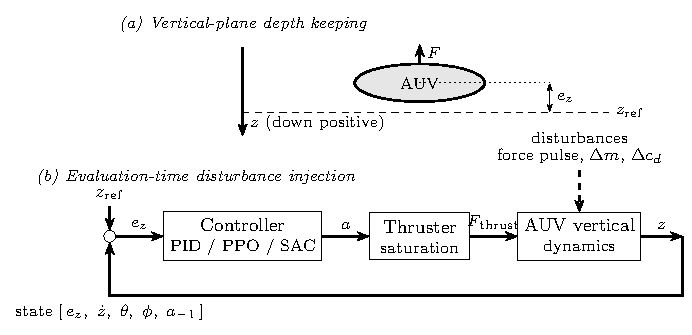
\includegraphics[width=\columnwidth]{fig1_system.pdf}
\caption{System overview: (a) vertical-plane depth-keeping task; (b) evaluation-time disturbance injection into the control loop.}
\label{fig:system}
\end{figure}

\subsection{Problem Formulation}
We formulate the AUV depth control problem as a depth-keeping task. The objective is to maintain the vehicle within $\pm 0.05$~m of the target depth for the full episode (500 steps). Performance is measured by the \textit{hold ratio}, defined as the fraction of steps within the target band. The system is illustrated in Fig.~\ref{fig:system}.

The vertical dynamics are modeled as a second-order system:
\begin{equation}
\ddot{z} = \frac{F_{\text{thrust}} + F_{\text{ext}} - c_d \dot{z}}{m},
\label{eq:dynamics}
\end{equation}
where $z$ is the depth, $m$ is the vehicle mass, $c_d$ is the drag coefficient, $F_{\text{thrust}} \in [-1, 1]$ is the normalized thruster command, and $F_{\text{ext}}$ is the external disturbance force.

\paragraph{Derivation and assumptions.} The vertical motion of a thruster-driven AUV can be written, in the body frame, as $m\ddot{z}_{\text{body}} = F_{\text{thrust}} + F_{\text{buoyancy}} + F_{\text{gravity}} + F_{\text{drag}} + F_{\text{ext}}$. Three standard simplifications reduce this to Eq.~\eqref{eq:dynamics}. First, we assume neutral buoyancy, so $F_{\text{buoyancy}} + F_{\text{gravity}} \approx 0$ over the operating depth range considered here (0--5\,m). Second, the hydrodynamic drag on the vertical axis is modeled as linear in the vertical velocity, $F_{\text{drag}} = -c_d \dot{z}$, which is a standard linearization valid for the low-speed regime ($|\dot{z}| \lesssim 0.5$\,m/s) typical of depth-keeping; a quadratic term $-c_d |\dot{z}|\dot{z}$ would refine accuracy at higher speeds but is not exercised by the present task. Third, we restrict attention to the vertical plane and treat pitch and roll as decoupled, small-amplitude perturbations: this is justified by the near-neutral buoyancy of the vehicle and the small thruster forces required for depth-keeping, which together keep attitude transients well below the $30^{\circ}$ soft limit (see the State, Action, and Termination subsection). The external disturbance $F_{\text{ext}}$ aggregates unmodeled effects (currents, tether loads, and impulsive perturbations) and is injected as force pulses in the experiment (see the Disturbance Injection subsection). The normalization $F_{\text{thrust}} \in [-1,1]$ maps the commanded thruster input to the physical force via the maximum thrust $F_{\max}$.

\subsection{State, Action, and Termination}
The observation is a 5-dimensional vector $[e_z, \dot{z}, \theta, \phi, a_{-1}]$, where $e_z$ is the depth error, $\dot{z}$ the vertical velocity, $\theta$ and $\phi$ the pitch and roll angles, and $a_{-1}$ the previous action. The action is the normalized thruster command $a_t \in [-1, 1]$. Episodes are always run for the full 500 steps and truncated thereafter; no early termination is applied. A step-wise hold bonus is granted whenever $|e_z| < 0.05$~m, which directly yields the hold ratio as the fraction of in-band steps per episode. Attitude limits ($|\theta|, |\phi| > 30^{\circ}$) are enforced as soft constraints via clipping and a fixed penalty; in the vertical-plane model used here, attitude transients do not reach the limit, and the constraint is retained for generality. The depth is clamped to $[0, 6]$~m, with the vertical velocity projected at the bounds.

\subsection{Reward Design}
The reward at each step is:
\begin{equation}
r_t = -\left(w_1 |e_t| + w_2 |\dot{z}_t| + w_3 |a_t| + w_4 |\Delta a_t|^2\right) + r_{\text{hold}},
\end{equation}
where $e_t = z_{\text{target}} - z_t$ is the depth error, $a_t$ is the action, and $\Delta a_t = a_t - a_{t-1}$. The hold bonus is:
\begin{equation}
r_{\text{hold}} = \begin{cases}
+1, & \text{if } |e_t| < 0.05, \\
0,  & \text{otherwise.}
\end{cases}
\end{equation}
The weight vector is $w = [1.0, 0.1, 0.01, 0.001]$.

\subsection{Reward Weight Selection}
The penalty weights $w = [1.0, 0.1, 0.01, 0.001]$ follow a decade-decay principle. The depth-error term ($w_1 = 1.0$) dominates, making tracking accuracy the primary objective; the velocity penalty ($w_2 = 0.1$) provides damping one order of magnitude weaker, suppressing oscillation without discouraging the approach transient; the action-magnitude penalty ($w_3 = 0.01$) acts as a weak energy proxy; and the action-increment penalty ($w_4 = 0.001$) regularizes control smoothness. Under typical operating magnitudes ($|e| \approx 5\times10^{-2}$\,m, $|\dot{z}| \approx 5\times10^{-2}$\,m/s, $|a| \approx 0.2$, $|\Delta a| \approx 5\times10^{-2}$), every weighted penalty is at least an order of magnitude smaller than the $+1$ hold bonus, so the bonus dominates the asymptotic return while the penalties shape the transient. We note that these shaping terms are heuristic rather than potential-based~\cite{ng1999shaping}; a sensitivity analysis over $w$ (see the Reward-Weight Sensitivity subsection) shows high and comparable critic explained variance across three weightings, supporting the robustness of the reported conclusions, while a fully systematic study of reward-weight interactions is left to future work.

\subsection{Reinforcement Learning Algorithms}
Two state-of-the-art DRL algorithms are evaluated: PPO~\cite{schulman2017ppo} and SAC~\cite{haarnoja2018sac}. Both agents share the same observation space, action space, and reward function, and both use observation normalization (running mean and standard deviation, clipped at 10) with unnormalized rewards. We retain each algorithm's reference network architecture: SAC uses an MLP with two hidden layers of 256 units (ReLU) for both actor and critic, whereas PPO uses separate actor and critic MLPs with two hidden layers of 64 units (tanh). Keeping the standard architectures avoids introducing a jointly tuned architectural confound, so the comparison reflects the algorithms as they are commonly deployed.

\textbf{PPO.} PPO is an on-policy method that constrains policy updates via a clipped surrogate objective:
\begin{equation}
L^{\text{PPO}} = \mathbb{E}_t\!\left[\min\!\left(\rho_t A_t,\, \text{clip}(\rho_t, 1{-}\epsilon, 1{+}\epsilon) A_t\right)\right],
\end{equation}
where $\rho_t = \pi_\theta(a_t|s_t) / \pi_{\theta_{\text{old}}}(a_t|s_t)$ is the importance ratio and $A_t$ the advantage estimate. We use $\epsilon = 0.2$ and GAE($\lambda = 0.95$).

\textbf{SAC.} SAC is an off-policy maximum-entropy method that maximizes both expected return and policy entropy:
\begin{equation}
J(\pi) = \sum_t \mathbb{E}_{(s_t, a_t) \sim \rho_\pi}\!\left[r(s_t, a_t) + \alpha\, \mathcal{H}(\pi(\cdot|s_t))\right],
\end{equation}
where $\alpha$ is a temperature parameter that is automatically tuned. The policy is trained with a replay buffer of $5\times10^5$ transitions, warmed up with $10^4$ random-action transitions before gradient updates begin.

\subsection{Domain Randomization}
To evaluate robustness to parameter uncertainty, domain randomization (DR) is applied during training. At each episode reset, the mass and drag coefficient are sampled as:
\begin{equation}
m \sim \mathcal{U}(0.9 m_0,\, 1.1 m_0), \quad c_d \sim \mathcal{U}(0.8 c_{d0},\, 1.2 c_{d0}),
\end{equation}
where $m_0$ and $c_{d0}$ are the nominal values. Observation noise $\mathcal{N}(0, 0.01)$ is added to the sensor readings during DR training.

\subsection{Disturbance Injection}
Force pulses are injected during training and evaluation as external disturbances:
\begin{equation}
F_{\text{ext}}(t) = \pm 0.3\,F_{\max} \quad \text{for } 1.0\,\text{s},
\end{equation}
applied at random times within the episode, never starting before step 100 (10\,s) so that the agent can settle near the target depth first; the pulse amplitude is further jittered by a factor drawn from $\mathcal{U}(0.8, 1.0)$ with random sign. Training uses 1--2 pulses per episode together with Gaussian observation noise $\mathcal{N}(0, 0.01)$; evaluation uses exactly 2 pulses per episode with observation noise disabled (see the Setup subsection).

\subsection{PID Baseline}
A PID controller serves as the classical baseline:
\begin{equation}
u(t) = K_p e(t) + K_i \int_0^t e(\tau) d\tau + K_d \frac{de(t)}{dt},
\end{equation}
with gains $K_p = 3.0$, $K_i = 0$, $K_d = 1.5$ selected by grid search on the nominal scenario. Higher gains were not pursued as they approach the aggressive tuning boundary impractical for real actuators.

\subsection{Evaluation Protocol}
All methods are evaluated under identical episode initializations (common random numbers, seed 5678), so episodes are paired across methods by construction. We therefore adopt the paired Wilcoxon signed-rank test as the primary statistical test, which accounts for the induced correlation and removes initial-condition variance---a standard variance-reduction practice in simulation comparison. Effect sizes are reported as rank-biserial correlation, and $p$-values are corrected for multiple comparisons using the Holm--Bonferroni procedure. All evaluations use 50 episodes per method per condition.

\section{Experiment}

\subsection{Setup}
\textbf{Environment.} All experiments use the normalized vertical-plane model of Section~III with unit mass $m_0 = 1.0$, drag coefficient $c_{d0} = 0.5$, and control period $\Delta t = 0.1$\,s; each episode lasts 500 steps (50\,s). At every reset, the initial depth is drawn from $\mathcal{U}(0, 5)$\,m, the target depth from $\mathcal{U}(1, 5)$\,m, the vertical velocity starts at zero, and the initial pitch is drawn from $\mathcal{U}(-0.1, 0.1)$\,rad. The hold band is $\pm 0.05$\,m around the target depth.

\textbf{Training configurations.} Five controllers are compared: the grid-tuned PID baseline, PPO trained in the nominal environment (PPO-nominal), PPO trained under force pulses with three seeds $\{0, 1, 2\}$ (PPO-pulse), PPO trained with domain randomization (DR-PPO), and SAC trained under force pulses (SAC-pulse); a nominally trained SAC (SAC-nominal) serves as a reference for the training-regime analysis. PPO variants are trained for $1.0\times10^{6}$ environment steps, SAC variants for $5.0\times10^{5}$ steps, and the three reward-weight variants of Table~\ref{tab:ablation} for $2.0\times10^{5}$ steps each. All policies are implemented with Stable-Baselines3 2.9.0 (Gymnasium 1.4.0, PyTorch 2.14.1, CPU); hyperparameters are listed in Table~\ref{tab:hyper}. SAC training curves are shown in Fig.~\ref{fig:training}.

\textbf{Perturbations at evaluation.} Each method is evaluated under four conditions: (i) nominal; (ii) force-pulse, with exactly two pulses per episode of magnitude $\pm 0.3\,F_{\max}$ (scaled by a factor drawn from $\mathcal{U}(0.8, 1.0)$, with random sign), each lasting 10 steps (1.0\,s), starting no earlier than step 100, and with observation noise disabled; (iii) mass offset $m = 1.15\,m_0$; and (iv) drag offset $c_d = 0.75\,c_{d0}$. The two offsets deliberately lie outside the DR training ranges (mass $\pm 10\%$, drag $\pm 20\%$), so they probe extrapolation rather than interpolation of the randomized policy.

\textbf{Protocol and metrics.} Every method--condition cell is evaluated over 50 episodes. Episode $i$ uses an explicit per-episode seed, so the $i$-th initial state is identical across methods and episodes are paired by construction (Section~III). Policies act deterministically, and the observation-normalization statistics are frozen from training. We report episode return, depth mean absolute error (MAE), and hold ratio---the fraction of in-band steps over the full 500-step episode, which is well defined because episodes end by truncation only (Section~III). All training and evaluation run on a CPU-only workstation (16 threads, WSL2 Ubuntu 22.04); PPO completes $1.0\times10^{6}$ steps in approximately 10 minutes, and SAC completes $5.0\times10^{5}$ steps in approximately 3 hours.

\begin{figure}[htbp]
\centering
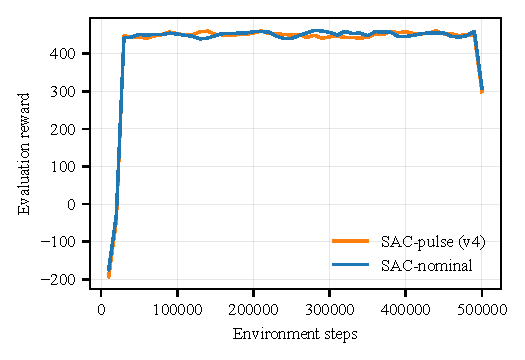
\includegraphics[width=\columnwidth]{fig2_training_curves.pdf}
\caption{Evaluation reward during training for SAC under two training regimes (pulse vs.\ nominal).}
\label{fig:training}
\end{figure}

\begin{figure}[htbp]
\centering
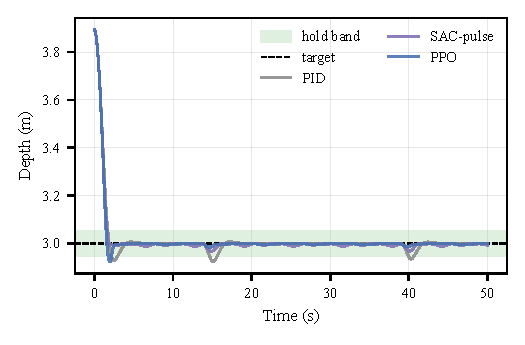
\includegraphics[width=\columnwidth]{fig3_trajectories.pdf}
\caption{Depth trajectories of all methods under the force-pulse evaluation scenario.}
\label{fig:traj}
\end{figure}

\begin{figure}[htbp]
\centering
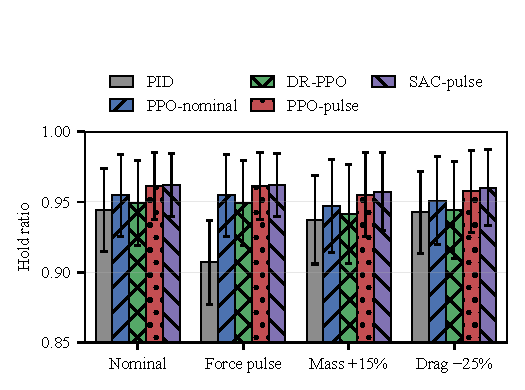
\includegraphics[width=\columnwidth]{fig4_robustness.pdf}
\caption{Hold-ratio comparison across nominal and perturbed conditions. The vertical axis is truncated to $[0.85, 1.0]$ for readability; all values lie within $0.90$--$0.97$.}
\label{fig:robust}
\end{figure}

\begin{figure}[htbp]
\centering
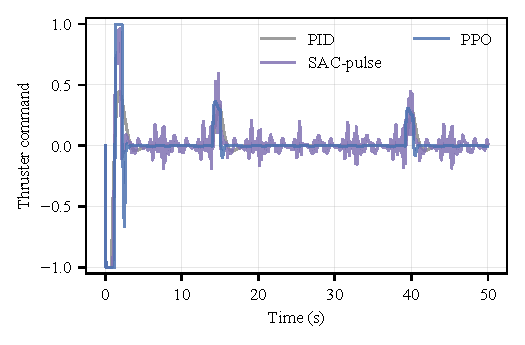
\includegraphics[width=\columnwidth]{fig5_actions.pdf}
\caption{Thruster command traces under the force-pulse scenario (smoothness comparison).}
\label{fig:actions}
\end{figure}

\subsection{Results}

\textbf{Nominal performance.} All methods solve the nominal task: hold ratios cluster within $0.944$--$0.962$ and nominal MAE within $0.047$--$0.051$\,m (Table~\ref{tab:nominal}), so differences on the undisturbed task are marginal. Two observations frame the rest of the analysis. First, the best nominal reward (PPO-pulse, $455.2$) and the best hold ratio (SAC-pulse, $0.962$) both come from pulse-trained agents, even though no pulses are present in this evaluation condition---the training-regime effect is therefore not specific to disturbed conditions. Second, for PPO the between-seed standard deviation ($0.002$ in hold ratio) is an order of magnitude smaller than the within-seed, episode-level standard deviation ($\approx 0.02$--$0.03$): episode initial conditions, not training seeds, dominate the variance budget. This observation motivates the paired evaluation design used throughout.

\textbf{Training regime.} Pulse-trained policies consistently outperform their nominal-trained counterparts across all four evaluation conditions, with hold-rate gains of 0.66--0.82 percentage points (paired Wilcoxon signed-rank test, $p < 0.001$ in all cases). This effect is systematic and consistent, though small relative to episode-to-episode variability. Fig.~\ref{fig:robust} summarizes the hold-ratio comparison across all conditions. Table~\ref{tab:stats} reports the paired statistical comparison.

\textbf{Domain randomization.} Domain randomization over mass $\pm 10\%$ and drag $\pm 20\%$ yields no benefit under the tested parameter offsets; it in fact incurs a small but statistically significant degradation of approximately 0.6 percentage points in hold ratio (paired Wilcoxon, $p < 0.001$). Notably, the evaluation offsets ($+15\%$ mass, $-25\%$ drag) lie outside the randomization ranges used during training, suggesting that the robustness conferred by DR does not extrapolate beyond the trained parameter distribution in our setup.

\textbf{Algorithm choice.} Training regime is the dominant factor in robustness; algorithm choice has only minor, condition-dependent effects. Under parameter offsets, SAC exhibits a small but significant edge over PPO (approximately 0.2 percentage points, $p < 0.05$), roughly $3$--$4\times$ smaller than the regime effect (approximately 0.7 percentage points).

\textbf{Control smoothness.} While SAC achieves a marginally higher hold ratio, it also produces notably larger action variations under the force-pulse scenario (mean $|\Delta a| \approx 0.068$, compared to 0.015 for PPO and 0.009 for PID; see Fig.~\ref{fig:actions}). This is consistent with prior reports that DRL controllers for AUVs tend toward aggressive, saturation-prone commands~\cite{du2023mrtd3}, and suggests that SAC adopts a more aggressive control strategy to exploit its entropy-regularized objective, whereas PPO attains comparable robustness with action profiles nearly as smooth as the classical PID baseline. For practical AUV deployment where actuator wear and energy consumption are key constraints, PPO's combination of robustness and smoothness may be preferable.

We emphasize that the regime and algorithm effects reported above are small in absolute terms (below one percentage point). Their interest lies in their consistency across all four evaluation conditions and in what they imply for evaluation methodology, rather than in a performance breakthrough.

\subsection{Reward-Weight Sensitivity}
To assess the sensitivity of the learned policies to the reward weights, we trained three PPO variants with the weight vectors listed in Table~\ref{tab:ablation} for $2\times10^5$ steps each, keeping all other hyperparameters fixed. Figure~\ref{fig:ablation} shows the critic's explained variance during training (the Stable-Baselines3 PPO implementation does not emit episode-return statistics under a purely-truncated environment). All three variants reach high explained variance by convergence (above $0.97$), indicating that the critic reliably predicts returns under each weighting and that the qualitative conclusions of this paper are not an artifact of a particular weight choice.

\begin{figure}[htbp]
\centering
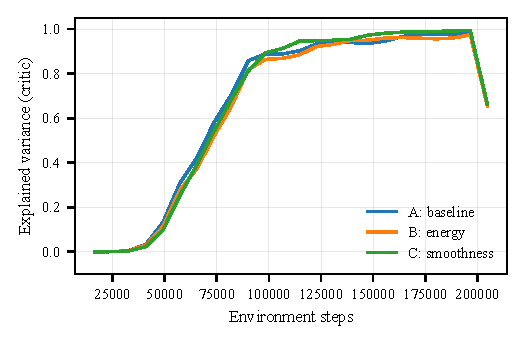
\includegraphics[width=\columnwidth]{fig6_ablation.pdf}
\caption{Reward-weight sensitivity: critic explained variance during training for three PPO variants (Table~\ref{tab:ablation}). All variants converge to high explained variance ($>0.97$).}
\label{fig:ablation}
\end{figure}

\subsection{Failure Analysis of the PID Baseline}
Since $K_i = 0$, the tuned baseline is effectively a PD controller, which exposes a structural weakness under constant-force disturbances. During a force pulse, cancelling the disturbance $F_{\text{ext}} = \pm 0.3\,F_{\max}$ requires a steady thrust command $|u^*| = 0.3$ (in normalized units, where $u = 1$ corresponds to $F_{\max}$). At equilibrium ($\dot{z} = 0$) the PD law settles at
\begin{equation}
|e_{\text{ss}}| = \frac{|u^*|}{K_p} = \frac{0.3}{3.0} = 0.10~\text{m},
\end{equation}
which is twice the half-width of the $\pm 0.05$\,m hold band. The vehicle therefore remains outside the band for the rest of each pulse and re-centers only after it ends. This first-principles estimate predicts at least $2 \times (10~\text{pulse steps} + \text{recovery}) \gtrsim 20$ lost hold steps per 500-step episode, i.e., a hold-ratio loss of $\gtrsim 4$ percentage points---consistent with the measured 3.7-point drop ($0.944 \rightarrow 0.907$, Table~\ref{tab:robust}).

Three classical remedies exist, and each was excluded for a concrete reason. Larger $K_p$ would shrink the offset but approaches the aggressive-tuning boundary that is impractical for real actuators (see the PID Baseline subsection). Integral action would eliminate the steady-state offset in principle, but it introduces windup risk while the thruster is saturated during the pulse, and the nominal-scenario grid search selected $K_i = 0$. Disturbance feedforward would cancel $F_{\text{ext}}$ directly, but it requires measuring the disturbance force, which is unavailable at deployment. Pulse-trained RL policies sidestep this dilemma by learning fast, large-magnitude counter-thrust responses to the pulse onset (Figs.~\ref{fig:traj} and~\ref{fig:actions}), maintaining a hold ratio of at least 0.955 under identical pulses.

\begin{table}[t]
\centering
\caption{Training and evaluation hyperparameters.}
\label{tab:hyper}
\begin{tabular}{@{}lcc@{}}
\toprule
 & \textbf{PPO (all variants)} & \textbf{SAC (v4)} \\
\midrule
Total env.\ steps   & $1.0\times10^{6}$ & $5.0\times10^{5}$ \\
Learning rate       & $3\times10^{-4}$  & $3\times10^{-4}$ \\
Batch size          & 64                & 256 \\
Discount $\gamma$   & 0.99              & 0.98 \\
Rollout / update    & 2048 steps, 10 epochs & 2 grad.\ steps/env.\ step \\
Entropy coefficient & 0 (fixed)         & auto-tuned \\
\midrule
\multicolumn{3}{@{}l@{}}{\textbf{Environment}: 500 steps/episode, hold band $\pm 0.05$\,m} \\
\multicolumn{3}{@{}l@{}}{\textbf{Pulse training}: $F{=}\pm0.3F_{\max}$, 1\,s, 1--2 per episode} \\
\multicolumn{3}{@{}l@{}}{\textbf{DR ranges}: mass $\pm10\%$, drag $\pm20\%$} \\
\multicolumn{3}{@{}l@{}}{\textbf{PID}: $K_p{=}3.0$, $K_i{=}0$, $K_d{=}1.5$ (grid search)} \\
\multicolumn{3}{@{}l@{}}{\textbf{Evaluation}: 50 paired episodes, common seed 5678} \\
\bottomrule
\end{tabular}
\end{table}

\begin{table*}[t]
\centering
\caption{Nominal performance over 50 paired episodes. Best value per column in bold; MAE lower is better. The PPO (3 seeds) row reports mean over three training seeds (std computed between seeds, $^{\dagger}$); all other rows report within-seed std over 50 episodes of a single training run.}
\label{tab:nominal}
\begin{tabular}{@{}lccc@{}}
\toprule
\textbf{Method} & \textbf{Reward} & \textbf{MAE (m)} & \textbf{Hold ratio} \\
\midrule
PID ($K_p{=}3.0$, $K_d{=}1.5$) & $445.96 \pm 43.80$ & $0.0484 \pm 0.0576$ & $0.944 \pm 0.029$ \\
PPO (3 seeds)$^{\dagger}$ & $450.74 \pm 1.95$ & $0.0494 \pm 0.0019$ & $0.955 \pm 0.002$ \\
DR-PPO        & $448.00 \pm 45.42$ & $0.0491 \pm 0.0592$ & $0.949 \pm 0.030$ \\
PPO-pulse     & $\mathbf{455.16 \pm 41.61}$ & $\mathbf{0.0473 \pm 0.0571}$ & $0.961 \pm 0.024$ \\
SAC-pulse (v4) & $453.16 \pm 40.64$ & $0.0512 \pm 0.0570$ & $\mathbf{0.962 \pm 0.023}$ \\
\bottomrule
\end{tabular}
\end{table*}

\begin{table*}[t]
\centering
\caption{Hold ratio under disturbance and parameter-offset scenarios (50 paired episodes each). Best per column in bold. All PPO and DR-PPO rows report seed 0; PID is deterministic. The 3-seed mean for the nominal PPO condition is given in Table~\ref{tab:nominal}.}
\label{tab:robust}
\begin{tabular}{@{}lcccc@{}}
\toprule
\textbf{Method} & \textbf{Nominal} & \textbf{Force pulse} & \textbf{Mass $+15\%$} & \textbf{Drag $-25\%$} \\
\midrule
PID         & 0.944 & 0.907 & 0.937 & 0.943 \\
PPO-nominal & 0.955 & 0.955 & 0.947 & 0.951 \\
DR-PPO      & 0.949 & 0.949 & 0.941 & 0.944 \\
PPO-pulse   & 0.961 & 0.961 & 0.955 & 0.958 \\
SAC-pulse (v4) & \textbf{0.962} & \textbf{0.962} & \textbf{0.957} & \textbf{0.960} \\
\bottomrule
\end{tabular}
\end{table*}

\begin{table*}[t]
\centering
\caption{Paired statistical comparison on hold ratio ($n{=}50$ paired episodes, common seed 5678). Diff: mean hold-ratio difference in percentage points, positive favoring the first-listed method. C1--C4 compare SAC-pulse (v4) against PPO-pulse (both trained under pulse injection). $r$: rank-biserial correlation. Holm $p$: Holm--Bonferroni corrected across the 12 tests.}
\label{tab:stats}
\begin{tabular}{@{}llccc@{}}
\toprule
 & \textbf{Comparison} & \textbf{Diff (pp)} & $r$ & \textbf{Holm $p$} \\
\midrule
A1 & PPO-pulse vs PID @ pulse     & $+5.42$ & $+1.00$ & $<0.001$ \\
A2 & SAC-pulse vs PID @ pulse     & $+5.51$ & $+1.00$ & $<0.001$ \\
\midrule
B1 & Regime @ nominal             & $+0.66$ & $+0.91$ & $<0.001$ \\
B2 & Regime @ pulse               & $+0.66$ & $+0.91$ & $<0.001$ \\
B3 & Regime @ mass $+15\%$        & $+0.82$ & $+0.93$ & $<0.001$ \\
B4 & Regime @ drag $-25\%$        & $+0.69$ & $+0.97$ & $<0.001$ \\
\midrule
C1 & SAC-pulse vs PPO-pulse @ nominal         & $+0.09$ & $+0.40$ & $0.209$ \\
C2 & SAC-pulse vs PPO-pulse @ pulse           & $+0.09$ & $+0.40$ & $0.209$ \\
C3 & SAC-pulse vs PPO-pulse @ mass $+15\%$    & $+0.22$ & $+0.59$ & $0.011$ \\
C4 & SAC-pulse vs PPO-pulse @ drag $-25\%$    & $+0.23$ & $+0.76$ & $0.002$ \\
\midrule
D1 & DR vs nominal @ mass $+15\%$ & $-0.57$ & $-1.00$ & $<0.001$ \\
D2 & DR vs nominal @ drag $-25\%$ & $-0.64$ & $-1.00$ & $<0.001$ \\
\bottomrule
\end{tabular}
\end{table*}

\begin{table}[t]
\centering
\caption{Reward-weight variants for sensitivity analysis.}
\label{tab:ablation}
\begin{tabular}{@{}lcccc@{}}
\toprule
Variant & $w_1$ & $w_2$ & $w_3$ & $w_4$ \\
\midrule
A (baseline)    & 1.0 & 0.1  & 0.01  & 0.001 \\
B (energy)      & 1.0 & 0.1  & 0.1   & 0.01  \\
C (smoothness)  & 1.0 & 0.01 & 0.001 & 0.1   \\
\bottomrule
\end{tabular}
\end{table}

\section{Discussion}
The effects we report are near the resolution limit of conventional evaluation. With an episode-level standard deviation of $\approx 0.03$ and $n=50$, a 0.7 pp difference corresponds to only $\approx 1.1$ standard errors under an unpaired design---consistent with our observation that the unpaired Welch $t$-test does not reach significance---so without common-random-number pairing, the regime effect is indistinguishable from initial-condition noise. We therefore regard paired evaluation not as an optional refinement but as a prerequisite for drawing any conclusion at this effect scale.

The same calculation quantifies the cost of ignoring pairing. Resolving a difference $\delta$ with an unpaired two-sample test at $k$ standard errors requires $n = 2(k\sigma/\delta)^2$ episodes per method; for $\sigma \approx 0.03$ and $\delta = 0.7$\,pp this gives $n \approx 150$ at $k{=}2$ and $n \approx 900$ at $k{=}5$, whereas our paired design reaches $p<0.001$ at $n=50$. Evaluation budgets of tens of episodes per method are common in practice, so sub-percentage-point regime or algorithm effects are systematically invisible to unpaired designs at such budgets; a non-significant unpaired result at this effect scale should be read as underpowered rather than negative.

We hypothesize that SAC's edge under parameter offsets stems from its entropy-regularized objective and off-policy replay: the former encourages smoother, less overcommitted policies, while the latter exposes the policy to a broader state distribution, both of which may improve tolerance to model mismatch. Verifying this mechanism is left to future work.

Our DR negative result is specific to the tested configuration. The randomization ranges ($\pm 10\%$ mass, $\pm 20\%$ drag) are narrower than the evaluation offsets, so the observed degradation may reflect an extrapolation failure rather than an intrinsic limitation of DR. Whether DR with ranges that cover the deployment deviations would provide a measurable benefit remains an open question, and is a natural direction for future work.

\subsection{Limitations}
Our study has three main limitations. First, the majority of trained agents are single-seed (except PPO, which uses three seeds); multi-seed replication would tighten the reported confidence intervals and strengthen the regime effect claim. Second, the dynamics are a simplified vertical-plane second-order model that omits lateral coupling, sensor dynamics, and actuator nonlinearities that are present on physical AUVs. Third, all evaluations are in simulation, without hardware validation; the sim-to-real gap may alter the absolute hold-ratio values, though the relative conclusions are expected to hold.

\subsection{Future Work}
Natural extensions include: (i) scaling to full 6-DOF dynamics with tether and current models, moving toward digital-twin-based validation pipelines~\cite{lin2025docking}; (ii) validation on physical AUV hardware in a controlled tank; (iii) investigating disturbance-aware critic architectures that explicitly model $F_{\text{ext}}$ as an auxiliary input; and (iv) adaptive DR schemes whose randomization range is updated online based on observed deployment deviations.

\section{Conclusion}
We presented a variance-reduced comparison of PID, PPO, and SAC for AUV depth control under four evaluation scenarios. Our results show that training regime is the dominant factor in robustness: pulse-trained policies consistently improve hold ratio by approximately 0.7 percentage points (paired Wilcoxon, $p<0.001$), whereas algorithm choice contributes less than 0.25 percentage points. Domain randomization within the tested ranges provides no benefit under parameter offsets outside those ranges, and PPO achieves robustness comparable to SAC with markedly smoother control actions. Future work includes extending the environment to 6-DOF, validating on physical AUV hardware, and investigating disturbance-aware critic architectures.

\bibliographystyle{IEEEtran}
\bibliography{refs}

\end{document}